\section{Results}
\label{framework:results}
The reason for performing the first experiment with the AnnotateMe Interface was to find out whether our approach of formulating and presenting the annotation data to a non-expert annotator for validation would result in creating high quality annotations. During this experiment we have also tested the performance of our NER service to see how well the recognition task is performed in addition to testing the performance of DBpedia Spotlight as the utilized automatic annotator. Below we report on the different aspects of the experiment.

\subsection{Participants}
The non-expert annotators who took part in the first experiment can be characterized as moderate users of text processing tools who have (on average) moderate experience with tagging of textual documents. Please note that tagging was explained to the users as the process of assigning a label or a textual description to a picture, video or categorizing a document. In some cases, the easiest way of explaining the tagging process to a participant was taking the concept of a \textit{hashtag} as an analogy to tagging. However, a \textit{hashtag} provides a higher degree of freedom since the tagging process is open while in our case the user is presented with options to choose from. Regardless, they both share the same conceptual idea. These questions were used to obtain a rough idea about the informal level of expertise of each participant in text processing respectively.

The average annotator was a 25 years old male student studying in the field of Computer Science with a good familiarity of text processing tools, moderate experience with tagging, acceptable level of familiarity with semantic web concepts who considered himself as above average when asked for his English language skills. Figure \ref{fig:ex1-preqestionnaire} presents the results of the questions asked to the participants during the pre-questionnaire. 

\begin{figure}[]
  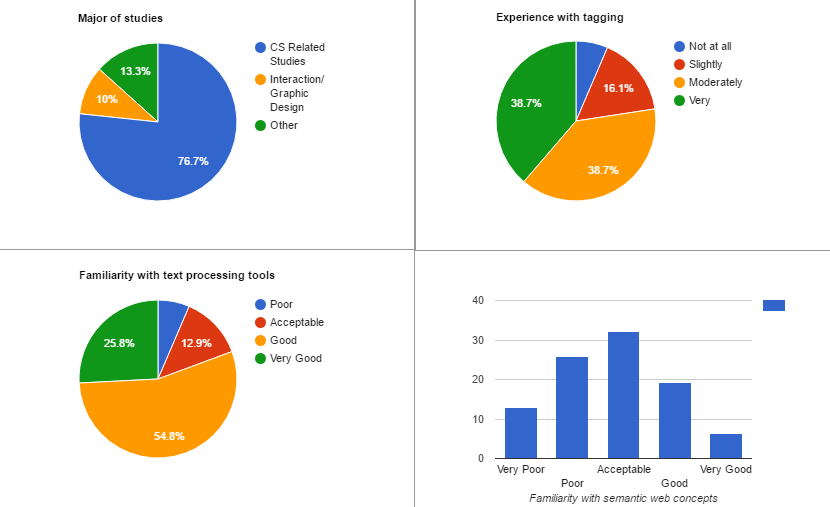
\includegraphics[width=\linewidth]{figures/experiment1/ex1-prequestionnairestats.PNG}
  \caption{Participant Statistics for Experiment 1}
  \label{fig:ex1-preqestionnaire}
\end{figure}

\subsection{NER Performance}
It has been mentioned earlier that the algorithms implemented in our \ac{ner} microservice are not novel solutions as opposed to the state-of-art. We attempted to reproduce the same algorithms used by \cite{39} since at the time of writing, their approach performed best compared to any other state-of-art \ac{ner} algorithms and tools. However, in absence of open source code, we tried to implement the service as similar as possible based on the information the authors provided in their white paper submitted at the OKE Challenge 2016 \cite{39}. As we can see from Table \ref{tab:ex1-nerperformance}, our framework performs significantly better than all the other automatic annotators for the KORE50 dataset, whereas for the spotlight we observe a slightly better improvement. Please note that we used GERBIL Benchmark \cite{40} to get the values for the other annotators whereas for our framework we calculated the same measures as explained by the benchmarking tool. 

% Table generated by Excel2LaTeX from sheet 'Sheet2'
\begin{table}[htbp]
  \centering
  \caption{NER Performance of automatic annotators in two datasets compared to our framework}
    \begin{tabular}{|l|ccc|ccc|}
    \toprule
    \textbf{-/Dataset} & \multicolumn{3}{c|}{\textbf{Spotlight Dataset}} & \multicolumn{3}{c|}{\textbf{KORE50 Dataset}} \\
    \midrule
          & \multicolumn{1}{l|}{\textbf{Precision}} & \multicolumn{1}{l|}{\textbf{Recall}} & \multicolumn{1}{l|}{\textbf{F-Score}} & \multicolumn{1}{l|}{\textbf{Precision}} & \multicolumn{1}{l|}{\textbf{Recall}} & \multicolumn{1}{l|}{\textbf{F-Score}} \\
    \midrule
    \textbf{Babelfy} & 0.22  & 0.18  & 0.19  & 0.55  & 0.55  & 0.53 \\
    \textbf{Dbpedia} & 0.61  & 0.34  & 0.43  & 0.73  & 0.23  & 0.27 \\
    \textbf{AIDA} & /     & /     & /     & 0.64  & 0.53  & 0.57 \\
    \textbf{Dexter} & 0.71  & 0.27  & 0.38  & 0.27  & 0.15  & 0.18 \\
    \textbf{AnnotateMe } & \textcolor[rgb]{ 1,  0,  0}{\textbf{0.69}} & \textcolor[rgb]{ 1,  0,  0}{\textbf{0.42}} & \textcolor[rgb]{ 1,  0,  0}{\textbf{0.49}} & \textcolor[rgb]{ 1,  0,  0}{\textbf{0.87}} & \textcolor[rgb]{ 1,  0,  0}{\textbf{0.8}} & \textcolor[rgb]{ 1,  0,  0}{\textbf{0.82}} \\
    \bottomrule
    \end{tabular}%
  \label{tab:ex1-nerperformance}%
\end{table}%

Our intentions were to see how good our framework performs when dealing with entities that have a very high ambiguous nature (KORE50 Dataset) but also with entities that have moderate levels of ambiguity (Spotlight Dataset). However, the number of entities present in each dataset was relatively big and resolving all of those entities using the framework would require running the experiment for longer periods. Therefore we used only a subset of documents from the Spotlight Dataset wheres for the KORE50 dataset we used all the available documents. For reproducability reasons, the following documents from the Spotlight dataset were considered: Arts1, Business1, Fashion1, Medicine1, Music1, Privacy1, Science1, Sports1, Travel1 and Travel2. The complete dataste is available online at the GERBIL website \footnote{\url{http://aksw.org/Projects/GERBIL.html}}. The total number of recognized entities by our NER microservice was 208 with 77 being entities recognized from the Spotlight dataset and 131 entities recognized from the KORE50 dataset.


\subsection{Annotation Quality and Performance}
Among the 208 total recognized entities by our \ac{ner} microservice, only 82 of them were resolved during the first experiment. It should be emphasized again that for one entity to be resolved we required 4 unique judgements from different participants to agree on one specific candidate for it to be resolved. We measured the performance of the human annotators, DBpedia Spotlight and other automatic annotators on those 82 resolved entities and evaluated whether the candidate associated with the entity was the correct one based on the gold standard. Additionally, since we wanted to see how DBpedia Spotlight (as our utilized automatic annotator) disambiguates entities based on the amount of contextual information surrounding the target entity, we report on three cases, namely: providing only the entity itself without any context information, providing the complete sentence and providing the contextual clues extracted from our framework. 
% Table generated by Excel2LaTeX from sheet 'Sheet3'
\begin{table}[htbp]
  \centering
  \caption{Annotation Results of AnnotateMe Interface and Dbpedia Spotlight Anntator}
    \begin{tabular}{|cc|cc|}
    \toprule
    \multicolumn{4}{|c|}{\textbf{Experiment 1 (Entity Name Only)}} \\
    \midrule
    \multicolumn{1}{|r|}{} & \multicolumn{1}{l|}{\textbf{All Datasets}} & \multicolumn{1}{l|}{\textbf{Spotlight Only}} & \multicolumn{1}{l|}{\textbf{KORE50 Only}} \\
    \midrule
    \multicolumn{1}{|c|}{\textbf{Correct (\%)}} & \multicolumn{1}{r|}{44.57} & \multicolumn{1}{r|}{72.22} & \multicolumn{1}{r|}{32.23} \\
    \multicolumn{1}{|c|}{\textbf{Incorrect (\%)}} & \multicolumn{1}{r|}{55.43} & \multicolumn{1}{r|}{27.78} & \multicolumn{1}{r|}{67.77} \\
    \midrule
    \multicolumn{4}{|c|}{} \\
    \midrule
    \multicolumn{4}{|c|}{\textbf{Experiment 1 (With Sentances)}} \\
    \midrule
    \multicolumn{1}{|r|}{} & \multicolumn{1}{l|}{\textbf{All Datasets}} & \multicolumn{1}{l|}{\textbf{Spotlight Only}} & \multicolumn{1}{l|}{\textbf{KORE50 Only}} \\
    \midrule
    \multicolumn{1}{|c|}{\textbf{Correct (\%)}} & \multicolumn{1}{r|}{51.38} & \multicolumn{1}{r|}{70.37} & \multicolumn{1}{r|}{43.31} \\
    \multicolumn{1}{|c|}{\textbf{Incorrect (\%)}} & \multicolumn{1}{r|}{48.62} & \multicolumn{1}{r|}{29.63} & \multicolumn{1}{r|}{56.69} \\
    \midrule
    \multicolumn{4}{c}{} \\
    \midrule
    \multicolumn{4}{|c|}{\textbf{Experiment 1 (With Context Clues \& Neighbor Entities)}} \\
    \midrule
    \multicolumn{1}{|r|}{} & \multicolumn{1}{l|}{\textbf{All Datasets}} & \multicolumn{1}{l|}{\textbf{Spotlight Only}} & \multicolumn{1}{l|}{\textbf{KORE50 Only}} \\
    \midrule
    \multicolumn{1}{|c|}{\textbf{Correct (\%)}} & \multicolumn{1}{r|}{54.24} & \multicolumn{1}{r|}{66.67} & \multicolumn{1}{r|}{48.78} \\
    \multicolumn{1}{|c|}{\textbf{Incorrect (\%)}} & \multicolumn{1}{r|}{45.76} & \multicolumn{1}{r|}{33.33} & \multicolumn{1}{r|}{51.22} \\
    \midrule
    \multicolumn{4}{|c|}{} \\
    \midrule
    \multicolumn{4}{|c|}{\textcolor[rgb]{ 1,  0,  0}{\textbf{AnnotateMe}}} \\
    \midrule
    \multicolumn{2}{|c|}{\textcolor[rgb]{ 1,  0,  0}{\textbf{Correct (\%)}}} & \multicolumn{2}{c|}{\textcolor[rgb]{ 1,  0,  0}{\textbf{Incorrect (\%)}}} \\
    \midrule
    \multicolumn{2}{|c|}{\textcolor[rgb]{ 1,  0,  0}{\textbf{88.46}}} & \multicolumn{2}{c|}{\textcolor[rgb]{ 1,  0,  0}{\textbf{11.53}}} \\
    \bottomrule
    \end{tabular}%
  \label{tab:exp1-annotatorRes}%
\end{table}%


Table \ref{tab:exp1-annotatorRes} presents the ratio of correctly and incorrectly linked entities by Dbpedia Spotlight. In general, the performance increased after providing more contextual information to the automatic annotator, which is an expected outcome. However, against our expectations, in the case of Spotlight Dataset, the ratio of correctly linked entities decreased after providing additional context information to the annotator. Despite the fact that the difference between the groups is not statistically significant for p < 0.5, it leads us to the assumption that Dbpedia Spotlight requires more content than just short contextual clues in order to make use of their internal techniques for disambiguation such as link probability, commonness, semantic similarity and other vector features relevant to context. Finally, we compare our performance results with other automatic annotators aside from Spotlight and we observe a significant improvement on both datasets. Table \ref{tab:exp1-annotatos-comparison} reports on the F-score of each annotator compared to our framework. 

Additionally, we run one-way Anova analysis of variance between two groups, namely, annotation results performed by non-expert users using the AnnotateMe Interface and results obtained by Dbpeida Spotlight automatic annotator. Statistically significant differences for p = 0.05 are obtained. As a result we claim that the non-expert annotators performed significantly better compared to other semantic annotators with an observed accuracy of 0.92 for the f-measure. Based on these results, the first hypothsis (H1.1) is strongly supported.

% Table generated by Excel2LaTeX from sheet 'Sheet4'
\begin{table}[htbp]
  \centering
  \caption{Comparison of AnnotateMe with other state-of-art semantic annotators}
    \begin{tabular}{|l|r|r|r|}
    \toprule
    \multicolumn{4}{|c|}{\textbf{Precision, Recall, F-Scores (Spotlight \& KORE50 Dataset)}} \\
    \midrule
    \textbf{Annotator} & \multicolumn{1}{l|}{\textbf{Precision}} & \multicolumn{1}{l|}{\textbf{Recall}} & \multicolumn{1}{l|}{\textbf{F-Score}} \\
    \midrule
    \textcolor[rgb]{ .8,  0,  0}{\textbf{AnnotatMe}} & \textcolor[rgb]{ .8,  0,  0}{\textbf{0.95}} & \textcolor[rgb]{ .8,  0,  0}{\textbf{0.88}} & \textcolor[rgb]{ .8,  0,  0}{\textbf{0.92}} \\
    \midrule
    Babelfy & 0.56  & 0.46  & 0.51 \\
    \midrule
    Dbpedia Spotlight & 0.53  & 0.39  & 0.44 \\
    \midrule
    Dexter & 0.27  & 0.17  & 0.2 \\
    \midrule
    WAT   & 0.55  & 0.41  & 0.46 \\
    \bottomrule
    \end{tabular}%
  \label{tab:exp1-annotatos-comparison}%
\end{table}%

In order to answer our second research question regarding context and deciding whether to accept or reject our second hypothesis (H1.2), we asked participants in the post questionnaire whether the contextual clues were helpful during the annotation process. They were also asked whether they would prefer to have the complete sentence as a representative of the surrounding context of the entity or whether they would prefer the short context clues already provided in the annotation interface. The results from the post questionnaire analysis show that 66.67\% of the participants preferred the short context clues as opposed to the 31.25\% of the other group who said that they would prefer sentences instead. To see whether contextual clues really helped on the disambiguation process for those participants who approved them as helpful clues, we calculated the level of agreement of each participant. The level of agreement is a simple calculation that takes the number of correct entities resolved and divides it by the total number of annotations performed. Results show that from the group who agreed having short contextual clues rather than sentences, on average they agreed with other annotators 54.47\% of the time, while those who preferred sentences agreed on average 48.44\% of the time. We observe a slight improvement on the agreement level in this case. Figure \ref{fig:ex1-agreementlevel} presents the overall agreement levels of all participants who took part in the first experiment. The average agreement level for all participants is 51\%. Please note that this does not represent a 50-50 chances of agreeing with another participant. In most cases, when resolving an entity, each participant was presented with 8 options in addition to the 9th option being "none of the above". Therefore, a 51\% reported agreement level can be considered a good performance. However, the difference between the agreement level reported for the group who preferred context clues compared to those who preferred sentences is not statistically significant for p = 0.05 and as a result our second hypothesis is rejected. 

%agreement level
\begin{figure}[]
  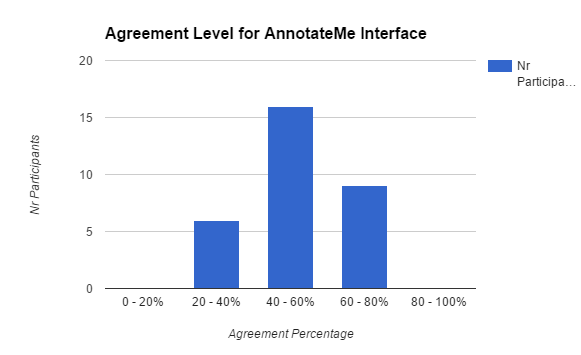
\includegraphics[width=\linewidth]{figures/experiment1/exp1-agreementlevel.PNG}
  \caption{Participants' Agreement level for the first experiment}
  \label{fig:ex1-agreementlevel}
\end{figure}
 

%freewill annotations
The setup of the first experiment was designed in a way that each individual participant performed annotations for 15 minuets constantly. They were not told upfront that they will be performing such tasks for 15 minutes, but were instructed to do the task until the experimenter told them to stop. After the estimated time elapsed they were asked whether they would like to continue do more annotations or stop and conclude the experiment. Participants were not encouraged to do any annotations after the 15 minute time trial had passed, thus the rest of annotations performed were completely voluntary and considered as free-will annotations. On average, each participant performed 22 annotation rounds during those 15 minutes. In terms of free-will annotations, one participant performed 17 annotation rounds on average. These results are used later to compare with the gamified system in order to assess the perceived engagement as a measure of time spent performing \textit{free-will annotating}. 

On the post questionnaire we asked participants to evaluate their experience with the task, the usability of the interface and perceived engagement. Figure \ref{fig:ex1-postresults} reports the results on the different questions asked on the post questionnaire. It can be concluded that the participants perceived the task to be interesting and somewhat engaging with a possibility that the participants would continue perform such task in the future. Regarding the usefulness of contextual clues, the graph indicates that users perceived the clues on average as useful when disambiguating a named entity. In addition to that, we report also on the perceived frustration while performing the task. Figure \ref{fig:ex1-frustration} indicates that the participants were seldom frustrated during the annotation process with some of the participants reporting to having been frustrated about half of the time. This can be an outcome of the participants being not familiar with the entities since they did not have the freedom of choosing a specific category or genre during the first experiment. 

%post questionnaire results 
\begin{figure}[]
  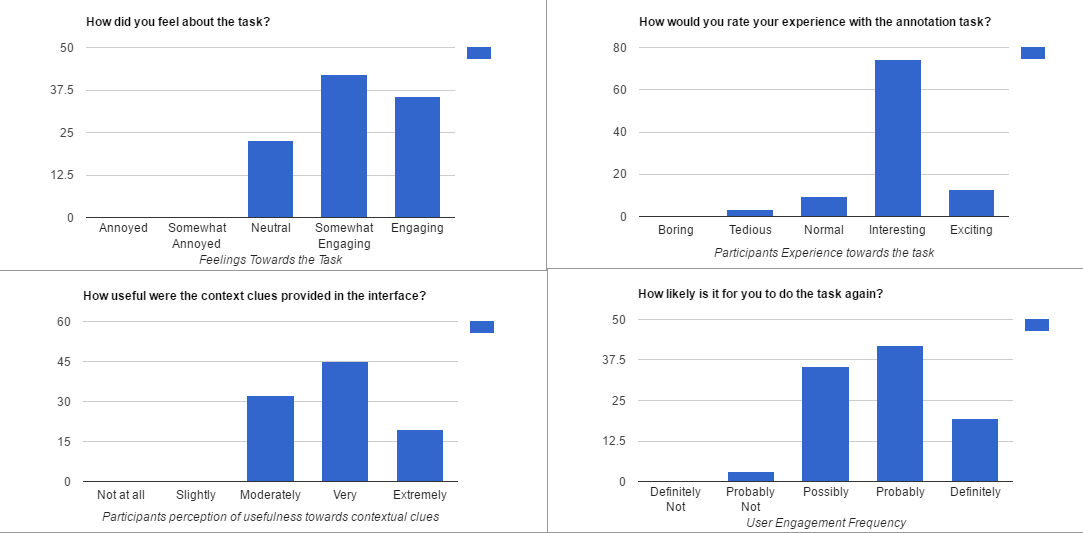
\includegraphics[width=\linewidth]{figures/experiment1/ex1-postquestionnaire.PNG}
  \caption{Experiment 1 Post Questionnaire Results}
  \label{fig:ex1-postresults}
\end{figure}

\begin{figure}[]
  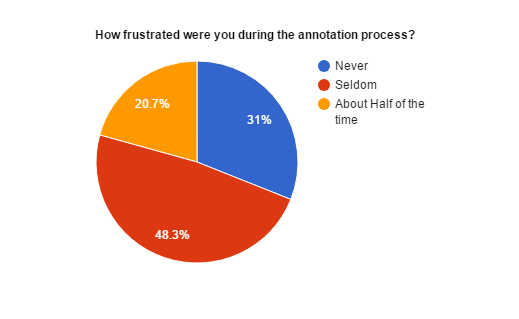
\includegraphics[width=\linewidth]{figures/experiment1/ex1-frustration.PNG}
  \caption{Reported level of frustration experienced during the annotation process}
  \label{fig:ex1-frustration}
\end{figure}

%Short contextual clues are preferred towards complete sentences or paragraphs and they provide sufficient information to make correct annotation decisions!